\subsection{基函数回归}
\label{sec:regression-basis}

OLS、岭、SVR等都在原始输入的线性空间里拟合；真实关系弯曲时，直线会在局部系统性偏高或偏低。\term{基函数回归}（basis function regression）先把原始输入通过一组固定函数映射到新特征，再在这些新特征上作线性拟合：系数仍然是线性的，非线性来自基函数本身。

\subsubsection{模型结构}
\label{sec:regression-basis-structure}

选取基函数$\phi_j:\mathbb{R}^d\to\mathbb{R}$（$j=1,\ldots,p$），把截距与基系数并成总参数$\bm{\theta}=(b,w_1,\ldots,w_p)^{\top}\in\mathbb R^{p+1}$、增广基向量$\widetilde{\bm{\phi}}(\bm{x})=(1,\phi_1(\bm{x}),\ldots,\phi_p(\bm{x}))^{\top}\in\mathbb R^{p+1}$，预测为
\begin{equation}
  f(\bm{x})=\widetilde{\bm{\phi}}(\bm{x})^{\top}\bm{\theta},
  \label{eq:regression-basis-model}
\end{equation}
其中待学对象是$\bm{\theta}$；基函数$\phi_j$本身、数量$p$与中心/结点先固定，模型结构本身尚未决定损失或概率假设。增广设计矩阵$\bm{\Phi}\in\mathbb{R}^{n\times(p+1)}$的第$i$行为$\widetilde{\bm{\phi}}(\bm{x}_i)^{\top}$；把式\eqref{eq:regression-ols-objective}中的特征列换成$\bm{\Phi}$后，OLS的平均半平方损失、梯度与系数求解全部原样复用（待学参数变为基系数与截距）。多项式与径向基是这一扩展的具体表示，下面分别展开；结点样条表示与平滑惩罚在GAM一节一起处理。

给定训练得到的$\widehat{\bm{\theta}}$与同一组基$\{\phi_j\}$（含其中心、结点等固定配置），对新输入$\bm{x}_\star$的实际预测规则为：按训练时的同一特征变换、中心和尺度计算$\widetilde{\bm{\phi}}(\bm{x}_\star)$，再代入式\eqref{eq:regression-basis-model}得$\widehat f(\bm{x}_\star)=\widetilde{\bm{\phi}}(\bm{x}_\star)^{\top}\widehat{\bm{\theta}}$。基的中心、半径、结点不得在新数据上重新估计或调整。

\subsubsection{参数学习}
\label{sec:regression-basis-learning}

采用平均半平方目标$J=(2n)^{-1}\sum_i e_i^2$，其中$e_i=f(\bm{x}_i)-y_i$。单样本随机梯度：对抽到的记录$i$，$\partial e_i/\partial w_j=\phi_j(\bm{x}_i)$、$\partial e_i/\partial b=1$，故单样本梯度为$e_i\phi_j(\bm{x}_i)$与$e_i$，更新为
\[
  w_j\leftarrow w_j-\eta\,e_i\phi_j(\bm{x}_i),
  \qquad
  b\leftarrow b-\eta\,e_i.
\]
批量形式即在全部样本上平均：$\partial J/\partial w_j=n^{-1}\sum_i e_i\phi_j(\bm{x}_i)$，截距同理，同一轮误差下同步更新。增广设计的直接最小二乘求解为$\bm{\Phi}^{\top}\bm{\Phi}\widehat{\bm{\theta}}=\bm{\Phi}^{\top}\bm{y}$；高阶多项式列之间高度相关，$\bm{\Phi}^{\top}\bm{\Phi}$条件数很大，可对基列中心化、正交化（如QR）或加入岭惩罚后求解，数值上避免直接求逆，秩亏时取最小范数解。若基函数中心或尺度也要学习，则需另外求相应导数，不能继续当成固定设计线性求解。

基参数（RBF中心与半径）通常先固定，再与基数量一起由训练内验证选择。

\subsubsection{多项式展开：增加曲率与交互}
\label{sec:regression-basis-polynomial}

\paragraph{多项式模型与系数学习}

$b+w_1x$无法表示斜率随输入改变的关系，局限来自特征表示，平方损失仍可使用。以$m(x)=x^2$为教学例，明确写出新模型$f(x)=b+w_1x+w_2x^2+\cdots+w_qx^q$，次数$q$是待选配置，$b,w_1,\ldots,w_q$是待学系数，对应设计行是$(1,x,\ldots,x^q)$。把一般梯度中的基函数换为$x_i^j$，即$\partial J/\partial w_j=n^{-1}\sum_i e_i x_i^j$，扩大设计后直接求解，不再重讲梯度下降的一般原理。一个可复算的小例：三个样本$(x,y)=(-1,1),(0,0),(1,1)$，取$q=2$，设计行依次为$(1,-1,1),(1,0,0),(1,1,1)$；由$\sum x_i^k$算得$\bm{\Phi}^{\top}\bm{\Phi}$的对角元为$(3,2,2)$、其余非零元为$\Phi_{0,2}=\Phi_{2,0}=2$，右端$\bm{\Phi}^{\top}\bm{y}=(2,0,2)^{\top}$，解得$\widehat b=0$、$\widehat w_1=0$、$\widehat w_2=1$，即$\widehat f(x)=x^2$，三个样本无误差。

图\ref{fig:regression-feature-approximation}给出一个教学投影例：设目标函数为$m(x)=x^2$、输入$X$在$[-1,1]$上均匀分布，问整个仿射候选空间$\{a+bx\}$中哪一个在平方积分意义下最接近$x^2$。由均匀分布矩$E[X]=0$、$E[X^2]=1/3$、$E[X^3]=0$、$E[X^4]=1/5$，正交投影的斜率为$\operatorname{Cov}(X,X^2)/\operatorname{Var}(X)=E[X^3]/E[X^2]=0$、截距为$E[X^2]=1/3$，故最佳仿射候选是常数$1/3$而非任意直线；其半积分平方误差为$\tfrac12 E[(X^2-1/3)^2]=\tfrac12(E[X^4]-1/9)=\tfrac{1}{2}(1/5-1/9)=2/45\approx0.0444$——图中阴影只表示两曲线的逐点差异，该数值是按上述矩算出的半均方误差，不是阴影的几何面积。

右图把候选空间放宽到$\{a+bx+cx^2\}$，$a=0,b=0,c=1$时$x^2$本身就在空间内，投影误差为零。两图都不是对有限样本的拟合，而是候选空间整体对目标的最近逼近：它区分表示误差（空间太小、任何样本都无法消除）与有限数据带来的估计、预测误差，为次数选择建立比较对象——只靠样本拟合无法看出空间本身是否装得下目标。

\begin{figure}[htbp]
  \centering
  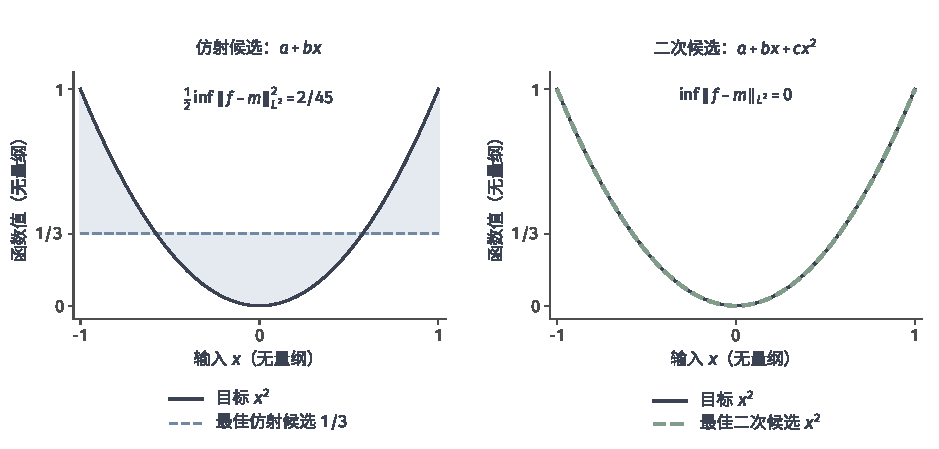
\includegraphics[width=105.412mm]{figures/07-classic-models/00-shared/matplotlib/regression-feature-approximation/figure.pdf}
  \caption{候选空间对目标$x^2$的整体投影（$X\sim\mathrm{Uniform}[-1,1]$）。左：仿射候选$\{a+bx\}$的最佳投影为常数$1/3$（斜率$0$），阴影为残差，$\tfrac12\inf\lVert f-m\rVert_{L^2}^2=2/45$；右：二次候选$\{a+bx+cx^2\}$包含$x^2$本身，投影误差为零。两图均不是有限样本拟合结果。}
  \label{fig:regression-feature-approximation}
\end{figure}

将单变量推广到多个输入时，以$x_1x_2$说明一个变量的作用可以随另一个变量改变。用多重指标$\bm{a}$与总次数$|\bm{a}|=\sum_ja_j$定义非恒定单项式$\bm{x}^{\bm{a}}=\prod_jx_j^{a_j}$，选$1\le|\bm{a}|\le q$形成设计列，$f(\bm{x})=b+\sum_{1\le|\bm{a}|\le q}w_{\bm{a}}\bm{x}^{\bm{a}}$，$\partial J/\partial w_{\bm{a}}=n^{-1}\sum_i e_i\bm{x}_i^{\bm{a}}$；交互项与单变量高次项的区别在此明确。

\paragraph{次数选择与外推}

比较嵌套的多项式空间，增加次数使最佳训练误差不增，却不能推出测试误差下降；多变量下增加总次数还会增加候选单项式数量，需要同时考虑样本与计算规模。因此在训练折构造特征并拟合，在验证折比较次数与正则强度。高次幂会带来数值放大，样本之外按最高次项发散，不能因训练区间内拟合改善就把结论外推到区间外。

\subsubsection{径向基：表达局部变化}
\label{sec:regression-basis-local}

\paragraph{径向基函数}

高次多项式影响整个区间，于是另一种思路是只在某些位置改变曲线，统一写$f(x)=b+\sum_jw_j\phi_j(x)$。\term{径向基}（RBF）取$\phi_j(\bm{x})=\exp(-\lVert\bm{x}-\bm{c}_j\rVert_2^2/(2r_j^2))$，每个中心$\bm{c}_j$只在附近隆起，组合后局部覆盖；中心$\bm{c}_j$与宽度$r_j$先固定，构建设计矩阵时沿用结构段的增广约定——第一列为常数$1$、其余列为$\Phi_{i,j+1}=\phi_j(\bm{x}_i)$，权重梯度把前节的$x_i^j$换成$\phi_j(\bm{x}_i)$，截距梯度不变。中心和宽度的选择只用训练数据及验证。

\paragraph{表示选择与配置}

两种表示职责不同：多项式基影响全局、次数决定曲率；RBF在中心附近局部隆起；分段样条基（结点附近弯曲、段间由导数条件保证光滑）在GAM一节与平滑惩罚一起展开。基数量增加意味着待估系数增多、估计方差上升，需要更多数据支撑；固定基不学习非线性参数，基的位置与形状本身是结构假设，选错基时系数再小也补不回来。多项式在训练区间之外按最高次项发散，外推不可靠；RBF在远离中心处归零，局部平滑但覆盖范围有限。选择应匹配任务在训练域内、外的要求，平滑惩罚由GAM进一步展开。
